\documentclass{beamer}
\usetheme{Boadilla}
\usepackage[utf8]{inputenc}
\usepackage{appendixnumberbeamer}
\setbeamercolor{alerted text}{fg=red!150!black!100}  %

\newcommand\gagnerduTemps[1]{#1}
\newcommand\XN{X^{(N)}}

\definecolor{green}{rgb}{0.0, 0.6, 0.0}
\definecolor{red}{rgb}{0.7, 0.0, 0.0}
\definecolor{blue}{rgb}{0.0, 0.0, 0.8}

\beamertemplatenavigationsymbolsempty
\usepackage{tikz}
\usepackage{mathtools}
\usepackage{appendixnumberbeamer}
\usetikzlibrary{shapes,arrows,positioning,automata}
\everymath{\displaystyle}

\newcommand\mpage[2]{%
  \begin{minipage}{#1\linewidth}%
    #2%
  \end{minipage}%
}

%%%%%%%%%%%%%%%%%%%%%%%%%%%%%%%%%%%%%%%%%%%%%%%%%%%%%%%%%%%%%%%%%%%%%%%%
%%% The following black magic puts copies of the table of contents
%%% throughout your talk: you might not want this.
\AtBeginSection[]
{
  \begin{frame}{Outline}
    \tableofcontents[current,currentsection]
  \end{frame}
}
%%%%%%%%%%%%%%%%%%%%%%%%%%%%%%%%%%%%%%%%%%%%%%%%%%%%%%%%%%%%%%%%%%%%%%%%


\newcommand\dt{\frac{d}{dt}}
\newcommand\esp[1]{\mathbb{E}\left[#1\right]}
\newcommand\var[1]{\mathrm{var}\left[#1\right]}
\graphicspath{{}{figures/}{../jsq2_simulate/}}

\definecolor{violet}{rgb}{0.3, 0., 0.2}
\setbeamercolor{math text}{fg=violet}
\newcommand\red[1]{{\color{red}#1}}
\newcommand\blue[1]{{\color{blue}#1}}
\newcommand\green[1]{{\color{green}#1}}
\newcommand\bx{\mathbf{x}}


\newcommand\bm{\mathbf{m}}
\newcommand\expect[1]{\mathbb{E}\left[#1\right]}
\newcommand\E{\mathbb{E}}
\newcommand\calS{\mathcal{S}}
\newcommand\calE{\mathcal{E}}
\newcommand\calA{\mathcal{A}}
\newcommand\calB{\mathcal{B}}
\newcommand\calT{\mathcal{T}}
\newcommand\calP{\mathcal{P}}
\newcommand\calL{\mathcal{L}}
\newcommand\Proba[1]{\mathbf{P}\left[#1\right]}
\newcommand\proba[1]{\mathbf{P}\left[#1\right]}
\newcommand\norm[1]{\left\|#1\right\|}
\newcommand\abs[1]{\left|#1\right|}
\newcommand\N{\mathbb{Z}^+}
\newcommand\R{\mathbb{R}}
\newcommand\bbm{\mathbf{m}}
\newcommand\bX{\mathbf{X}}
\newcommand\bE{\mathbf{E}}
\newcommand\LN{L^{(N)}}
\newcommand\bl{{\text{\boldmath$\ell$}}}

\DeclareMathOperator*{\argmin}{arg\,min}

\setbeamertemplate{blocks}[rounded][shadow=false]
\setbeamercolor*{block title}{fg=blue!70!black!90, bg=blue!8}
\setbeamercolor*{block body}{bg=blue!4}

\tikzset{every picture/.append style={shorten >=2pt,line width=2pt}}
\tikzstyle{wide}=[line width=2pt,->]

\makeatother
\setbeamertemplate{footline}
{
  \hfill 
  \usebeamerfont{author in head/foot}\insertshortauthor{} -- 
  \insertframenumber{} / \inserttotalframenumber\hspace*{1ex}
  \vskip0pt%
}
\makeatletter

\begin{document}

\title{Expected Values Estimated via Mean-Field Approximation are
  $1/N$-Accurate }%
\author{Nicolas Gast}%
\institute{Inria, Grenoble, France}%
\date[Urbana-Champaign, June 2017]{Sigmetrics 2017, Urbana-Champaign }%

\maketitle


\newcommand\newcite[3]{\item[#1] \textbf{#2} -- #3}

\newcommand\object[1]{\node[fill] at (#1) {~};}
\begin{frame}{What is mean-field approximation ?}
  {We study a population of $N$ interchangeable objects. }
  $\XN$ denotes the empirical measure.
  \begin{align*}
    \XN_i(t) = \text{ fraction of objects in state $i$ }
  \end{align*}
  

\end{frame}

\begin{frame}{Idea of mean-field: Some models simplify as
    $N\to\infty$}
  \begin{center}
    
    \mpage{.45}{
      \begin{exampleblock}{Theorem (Kurtz 70,\dots)}
        \centering $\displaystyle \XN(t) \approx x(t)$
      \end{exampleblock}
    }
  \end{center}
  
  \bigskip

  \begin{tabular}{cc}
    \mpage{.4}{
    Example: $N$ servers\\
    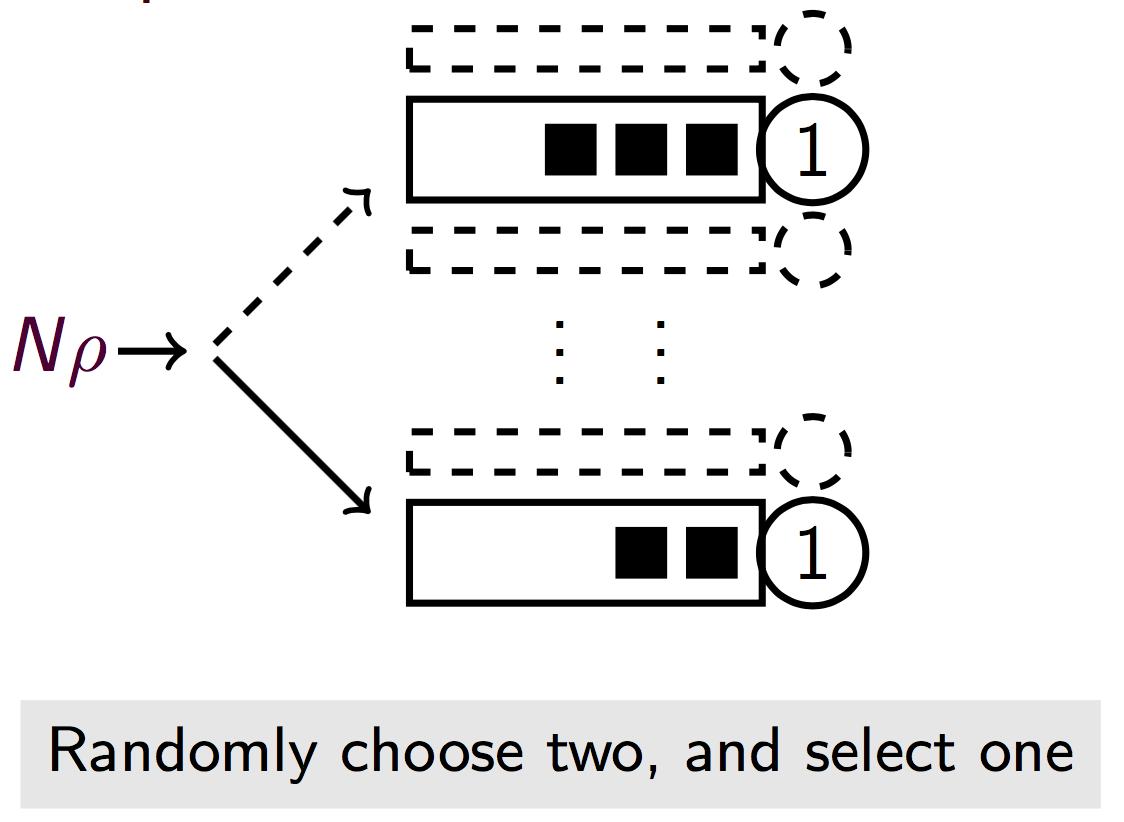
\includegraphics[width=\linewidth]{twoChoiceModel}
    }
 & 
   \mpage{.5}{
   \begin{tikzpicture}
     \node at (0,0){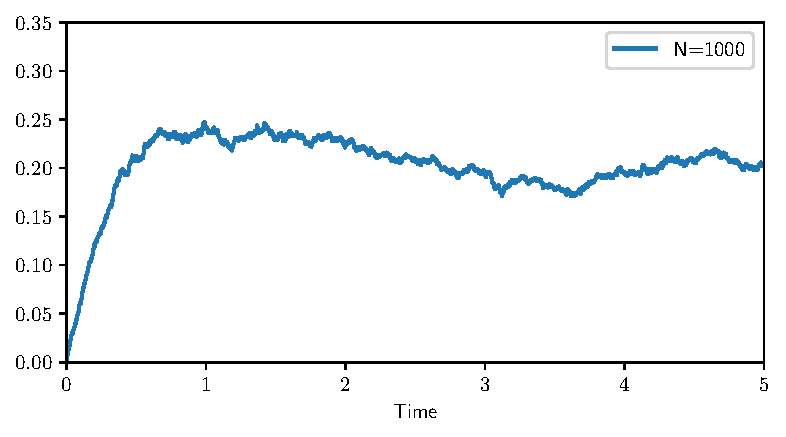
\includegraphics[width=\linewidth]{traj_rho80_onlyN1000}};
     \node at
     (0,-3){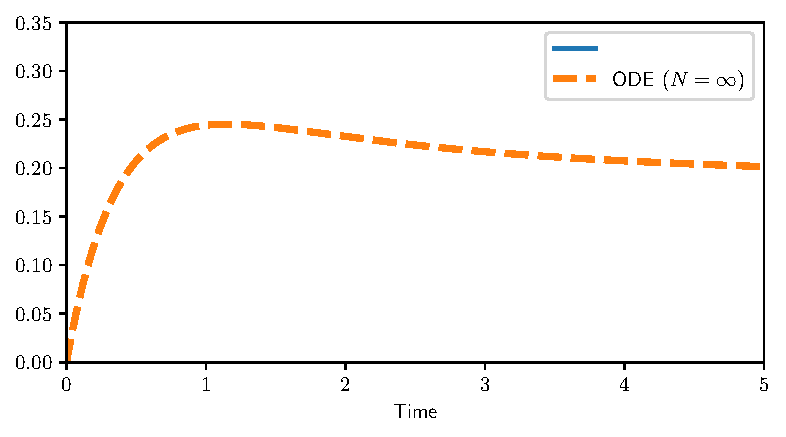
\includegraphics[width=\linewidth]{traj_rho80_onlyNinfty}};
     \uncover<3>{\node at
     (0,-3){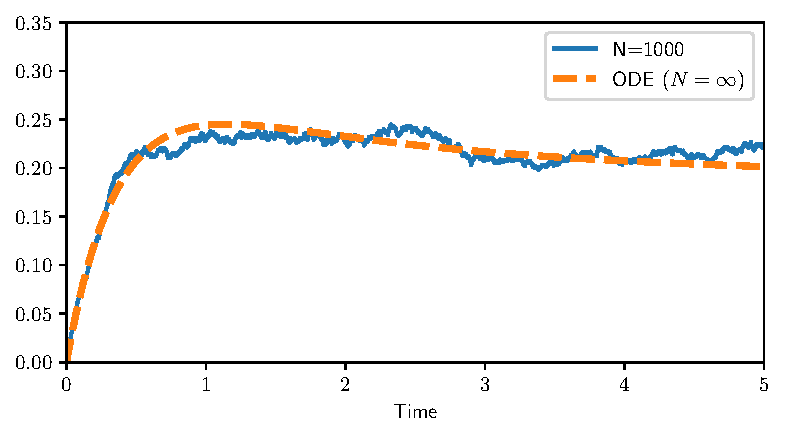
\includegraphics[width=\linewidth]{traj_rho80_onlyNinfty1000}};}
     \draw (0,-.5) edge[->,line width=2pt] node[right,fill=white] {$N\to\infty$}
     (0,-2); 
   \end{tikzpicture}
   }
  \end{tabular}
  
  
\end{frame}

\begin{frame}{Mean-field approximation is widely used in our
    community}{A few examples of recent SIGMETRICS papers\dots}
  
  \footnotesize 
  \begin{itemize}
  \newcite{2016}{ Asymptotics of Insensitive \red{Load Balancing} and Blocking
    Phases}{Jonckheere - Prabhu}
  \newcite{2016}{ On the Approximation Error of Mean-Field Models}{Ying}
  \newcite{2015}{ \red{Power of d Choices} for Large-Scale Bin Packing: A Loss
    Model}{Xie et al} 
  \newcite{2015}{ Transient and Steady-state Regime of a Family of
    List-based \red{Cache} Replacement Algorithms}{Gast, Van Houdt} 
  \newcite{2013}{  Queueing system topologies with limited
    flexibility.}{Tsitsiklis, Xu}
  \newcite{2013}{ A mean field model for a class of garbage collection
    algorithms in flash-based \red{solid state drives}.}{Van Houdt}
  \newcite{2012}{ Fluid limit of an asynchronous \red{optical packet switch} with shared per link full range wavelength conversion.}{Van Houdt,
    Bortolussi}

  \newcite{2011}{ On the power of (even a little) centralization in
    distributed processing. }
  \newcite{2010}{ Randomized load balancing with general service time
    distributions.}{Bramson et al.}
  \newcite{2010}{ \red{Incentivizing} peer-assisted services: a fluid shapley
    value approach.}{Misra et al}
  \newcite{2010}{ A mean field model of work stealing in large-scale
    systems.}{Gast, Gaujal} 
  \newcite{2009}{
The age of gossip: spatial mean field regime.}{Chaintreau et al.}
\item[$\vdots$~~]
  \end{itemize}
\end{frame}

\begin{frame}{\uncover<2->{\red{In theory},} how accurate is mean-field
    approximation?} 
  \pause
  \begin{center}
    
    \mpage{.45}{
      \begin{exampleblock}{Theorem (Kurtz 70\dots Ying 16) }
        \centering $\displaystyle \XN(t) \approx x(t) \red{+ \frac1{\sqrt{N}} G_t}$
      \end{exampleblock}
    }
  \end{center}
  
  \bigskip

  \begin{center}
    \mpage{.7}{
    \begin{tikzpicture}
      \uncover<3>{\node at (0,0) {\includegraphics[width=\linewidth]{traj_rho80_N10}};}
      \uncover<4>{\node at (0,0) {\includegraphics[width=\linewidth]{traj_rho80_N100}};}
      \uncover<5->{\node at (0,0) {\includegraphics[width=\linewidth]{traj_rho80_N1000}};}
       \draw[->] (-3.5,-2.1) -- (-3.5,3);
       \draw[->] (-3.5,-2.1) -- (4.5,-2.1);
       \node[fill=white] at (0,2.9) {$X_3(t)$ -- Fraction of servers with $3$ jobs};
       \node at (5,-2) {Time};
   \end{tikzpicture}
    }
  \end{center}
\end{frame}

\begin{frame}{\red{In practice}, how accurate is mean-field
    approximation?}{Can we use the approximation for $N=1000$?  
    $N=100$? $N=10$?} 
  
  \begin{table}[ht]
    \centering
    \begin{tabular}{|c|c|c|c|c|c|}
      \hline $N$&10&100&1000&$\infty$\\\hline
      Average queue length (simulation) & 2.8040	&2.3931	&2.3567	&2.3527\\%
      \only<1>{&&&&}\only<2->{Error of mean-field&      \red{0.4513}	&\red{0.0404}
                                        &\red{0.0040} &0}\\%
      \noalign{}\hline\noalign{}
    \end{tabular}    
    \caption{Two-choice model with $\rho=0.9$}
    \label{tab:avg}
  \end{table}
  
  \uncover<3->{
    Contributions : 
    \begin{enumerate}
    \item We show that, for \red{expected values}, the error of m-f is
      $O(1/N)$ under very general conditions
    \item In addition to previous work, the drift needs to be
      twice-differentiable.
    \item We study numerically the power-of-two choice. 
    \end{enumerate}
  }
\end{frame}




\begin{frame}{Outline}
  \tableofcontents
\end{frame}

\section{The Model (Kurtz's DDPP) and the Classical Convergence Results}

\begin{frame}{\uncover<2>{\red{Population}} CTMC}{\uncover<2>{Density
      dependent population process (70s)}} 
  \only<1>{A continous-time Markov chain (CTMC) with state-space $\bE$
    is given by an initial state $x_0$ and its transitions
    ($\ell\in\calL$):\\} \only<2>{A population process is a sequence
    of CTMC $\bX^N$, indexed by the \alert{population size $N$}, with
    state spaces $\bE^N\subset \bE$, with initial state $x_0$ and with
    transitions (for $\ell\in\calL$):}
\begin{align*}
    X \mapsto X+\uncover<1>{\ell}\uncover<2>{\red{\frac{\ell}{N}}} \qquad \text{ at rate
    $\uncover<2>{\red{N}}\beta_\ell(X)$}.
  \end{align*}
  
  \alert{The drift} is $f(x) = \sum_{\ell} \ell \beta_\ell(x)$.
  
  \phantom{\footnote{We assume $(\bE,\norm{\cdot})$ is a Banach space, not
    necessarily $\R^d$.}}
\end{frame}

\begin{frame}{Transient regime}
  Let $\Phi_t$ denotes the (unique) solution of the ODE : 
  \begin{align*}
    \Phi_tx &= x + \int_0^tf(\Phi_sx)ds.
  \end{align*}\pause 
  
  \begin{theorem}[Kurtz 70s]
    If $f$ is Lipschitz-continuous with constant $L$, then for any
    fixed $T$: 
    \begin{align*}
      \sup_{t<T}\norm{X^N(t) - \Phi_t X^N(0)} = O(1/\sqrt{N}) \qquad \xrightarrow{N\to\infty}0.
    \end{align*}
  \end{theorem}

  \begin{center}
    \mpage{.5}{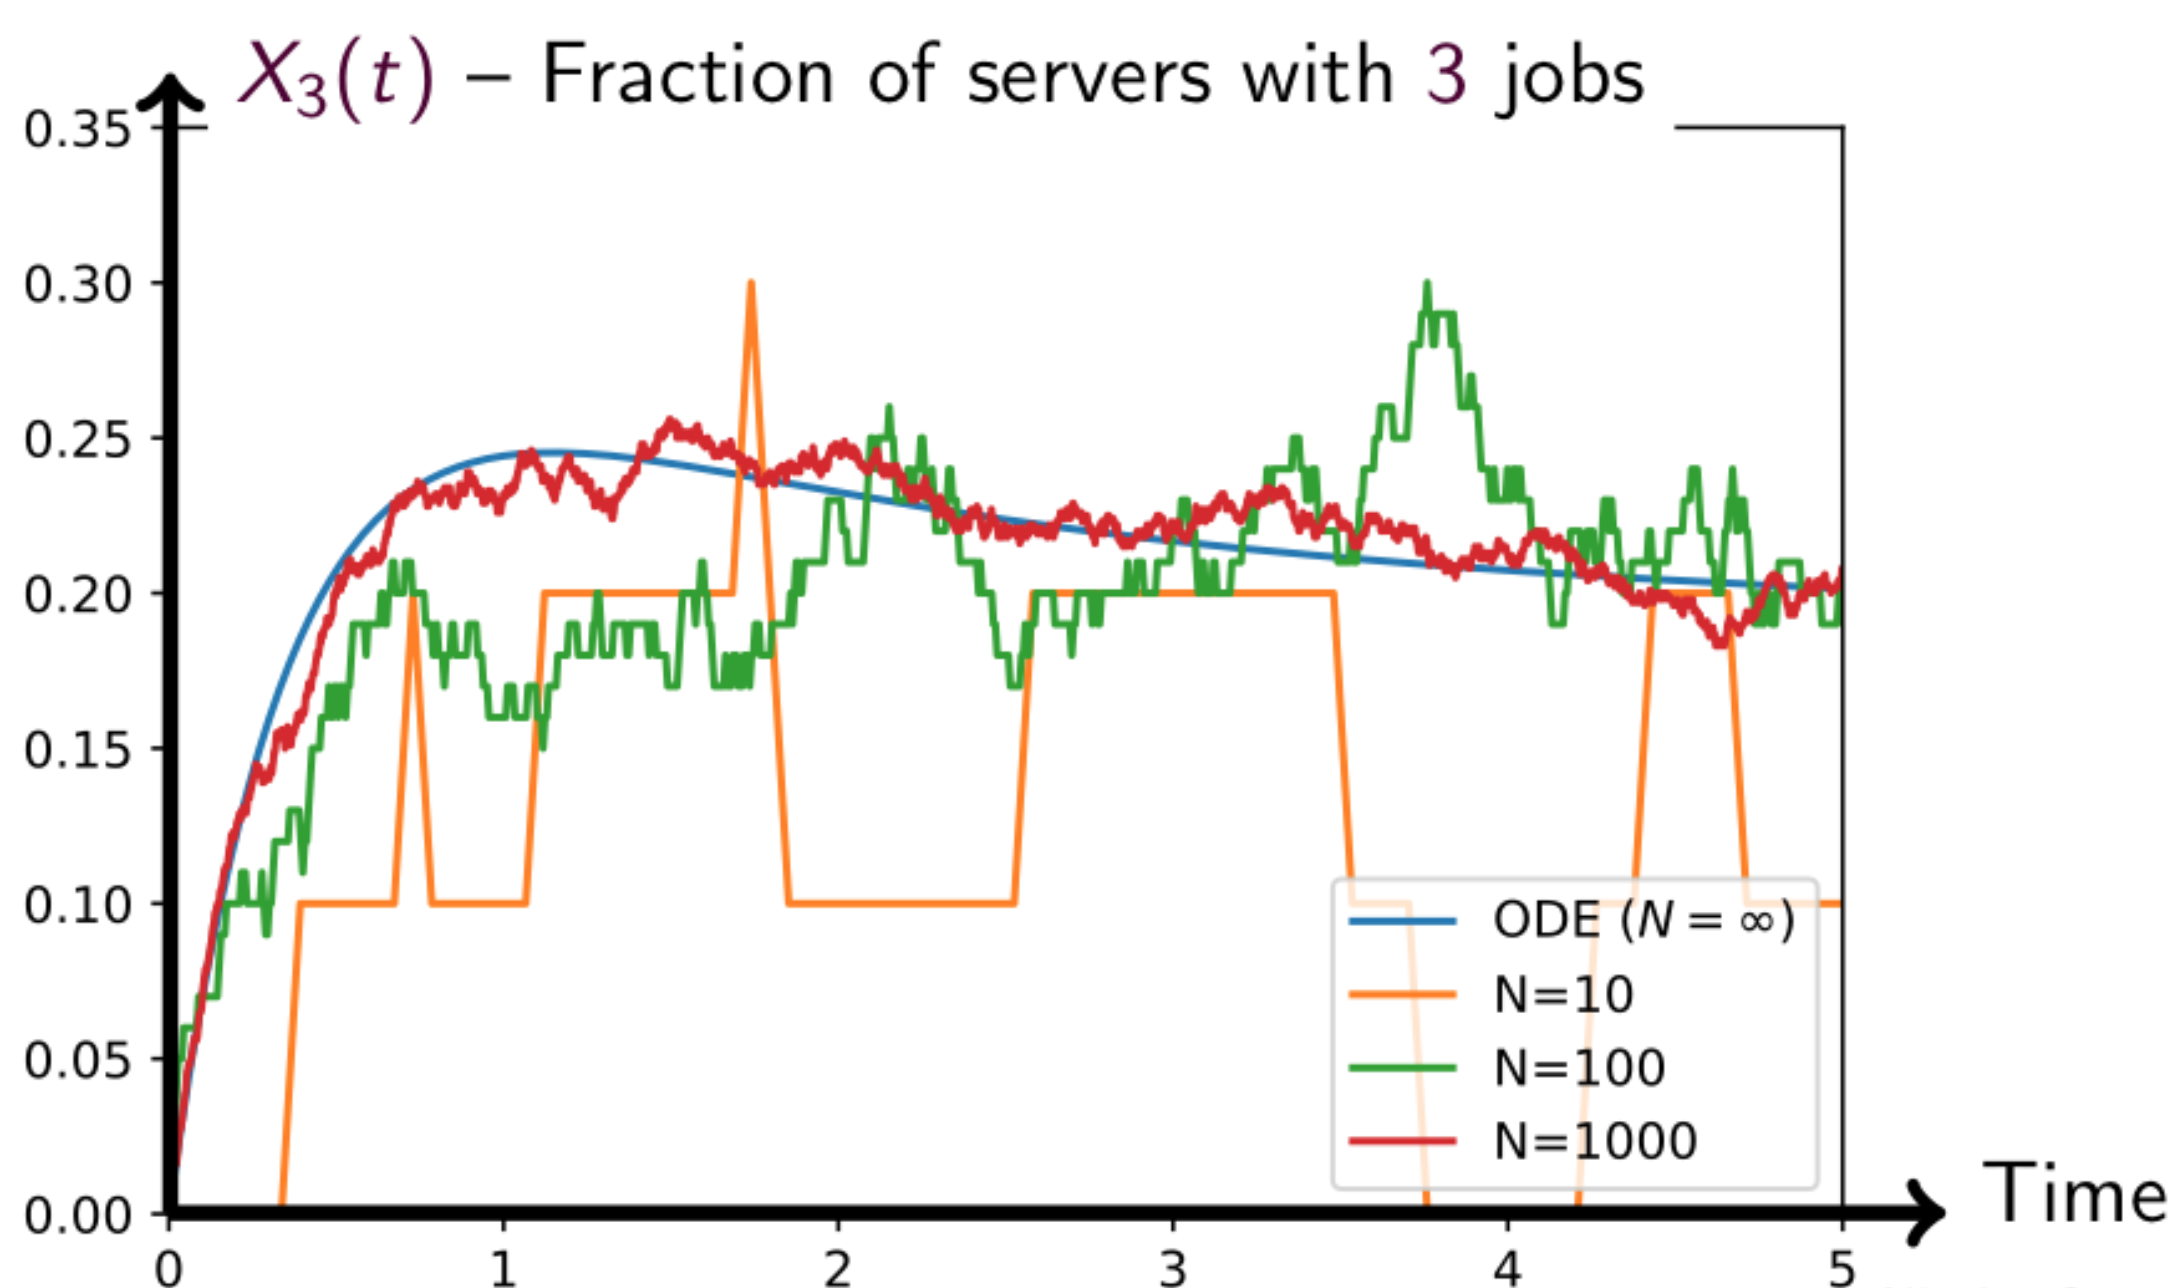
\includegraphics[width=\linewidth]{clt}}
  \end{center}

  
\end{frame}

\begin{frame}{Stationary regime}
  If the ODE $\dot{x}=f(x)$ has a unique fixed point $x^*$ that is
  exponentially stable, then:\bigskip
  \begin{theorem}[Ying 2016]
    If $f$ is Lipschitz-continuous with constant $L$, then for any
    fixed $T$: 
    \begin{align*}
      \esp{\norm{X^N - x^*}} = O(1/\sqrt{N}) \qquad \xrightarrow{N\to\infty}0.
    \end{align*}    
  \end{theorem}

  \bigskip Remark : The uniqueness of the fixed point is not
  sufficient, see Benaim-Le Boudec 2008.
\end{frame}


\section{The $O(1/N)$-Accuracy of Mean-Field Approximation}

\begin{frame}{$1/\sqrt{N}$ or $1/N$?}

  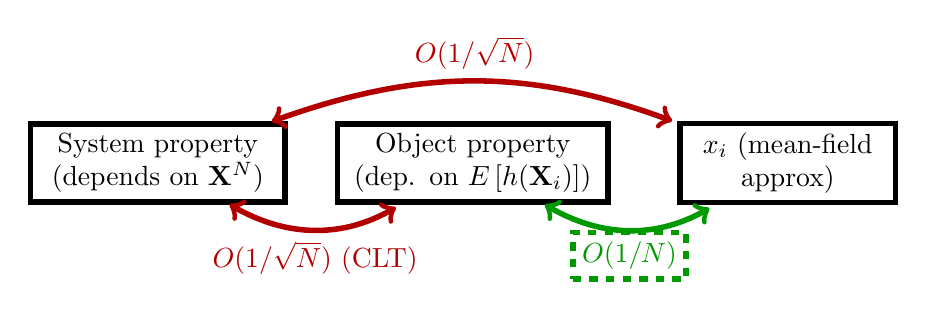
\begin{tikzpicture}
    \node[text width=3cm,draw,text centered] at (0,0) (X) {System
      property (depends on $\bX^N$)}; %
    \uncover<2->{%
      \node[text width=3.2cm,draw,text centered] at (4,0) (P)%
      {Object property\\ (dep. on $\esp{h(\bX_i)}$)}; %
    }%
    \node[text width=2.5cm,draw,text centered] at (8,0) (x) {$x_i$
      (mean-field approx)};%
    \uncover<1->{\draw[red,line width=2pt] (X) edge[bend
      left,<->,in=160,out=20] node[above]{$O(1/\sqrt{N})$} (x);}%
    \uncover<2->{\draw[red,line width=2pt] (X) edge[bend right,<->]
      node[below]{$O(1/\sqrt{N})$ (CLT)} (P);}%
    \uncover<2->{\draw[green,line width=2pt] (P) edge[bend right,<->]
      node[dashed,draw,below]{$O(1/N)$} (x);%
    }
  \end{tikzpicture}

  \begin{center}
    \begin{tabular}{|c|c|c|c|c|}
      \hline
      $N$ & 10 & 100 & 1000 &$+\infty$\\\hline
      Average queue length ($m^N$) &2.81&2.39&2.36& 2.35\\\hline
      Error ($m^N-m^\infty$) & 0.46 & 0.039 & 0.004 & 0 \\\hline
    \end{tabular}
  \end{center}
\end{frame}




\begin{frame}{Steady-state analysis}
  $\dot{x}=f(x)$ has an exponentially stable attractor $x^*$ if for
  any solution:
  \begin{align*}
    \norm{x(t)-x^*} \le C e^{-\alpha t}\norm{x(0)-x^*}.  
  \end{align*}
  
  \pause
  \begin{theorem}
    If $f$ is twice differentiable, if the ODE has an exponentially
    stable attractor $x^*$ and if there exists a bounded set $\calB$
    such that $\Proba{X^N\not\in \calB}=O(1/N^2)$, then for any
    bounded function $h$, there exists a constant $K$ such that:
    \begin{align*}
      \limsup_{N\to\infty}N\abs{\esp{h(X^N)} - h(x^*)} \le 
      K.
    \end{align*}
  \end{theorem}
  \begin{itemize}
  \item Note: A similar result holds for the transient behavior.
  \end{itemize}

\end{frame}

\begin{frame}{Main ideas of the proof}
  \textbf{1.} \red{Comparison of the generators}:
  \begin{align*}
    (\LN h) (x) &=\sum_{\ell\in\calL}N\beta_{\ell}(x)(h(x+\frac{\ell}{N}) - h(x) )\\
    (\Lambda h) (x) &= \sum_{\ell\in\calL}\beta_{\ell}(x)Dh(x)\cdot \ell
                      = Dh(x)\cdot f(x)
  \end{align*}

  \textbf{2.} \red{Stein's method} : 
  \begin{align*}
    \esp{h(X^N)-h(x^*)} = \esp{(\Lambda-\LN) (Gh) X^N},
  \end{align*}
  where $Gh(x) = \int_0^\infty (h(\Phi_tx) - h(x^*))dt$
  satisfies $h(x) - h(x^*) = \Lambda (Gh) x$. 
  \bigskip
  
  \textbf{3.} \red{Perturbation theory} shows that $D^2(Gh)$ is
  twice-differentiable.
\end{frame}


\section{Application Example: Two-Choice Model}

\begin{frame}{The two choice model\footnote{\tiny This model or
      variants have been heavily studied {\tiny (Vvedenskaya 96,
        Mitzenmacher 98 \dots Tsitsiklis et al. 2016,\dots)}.}}
  \begin{tabular}{cc}
    \mpage{.45}{
    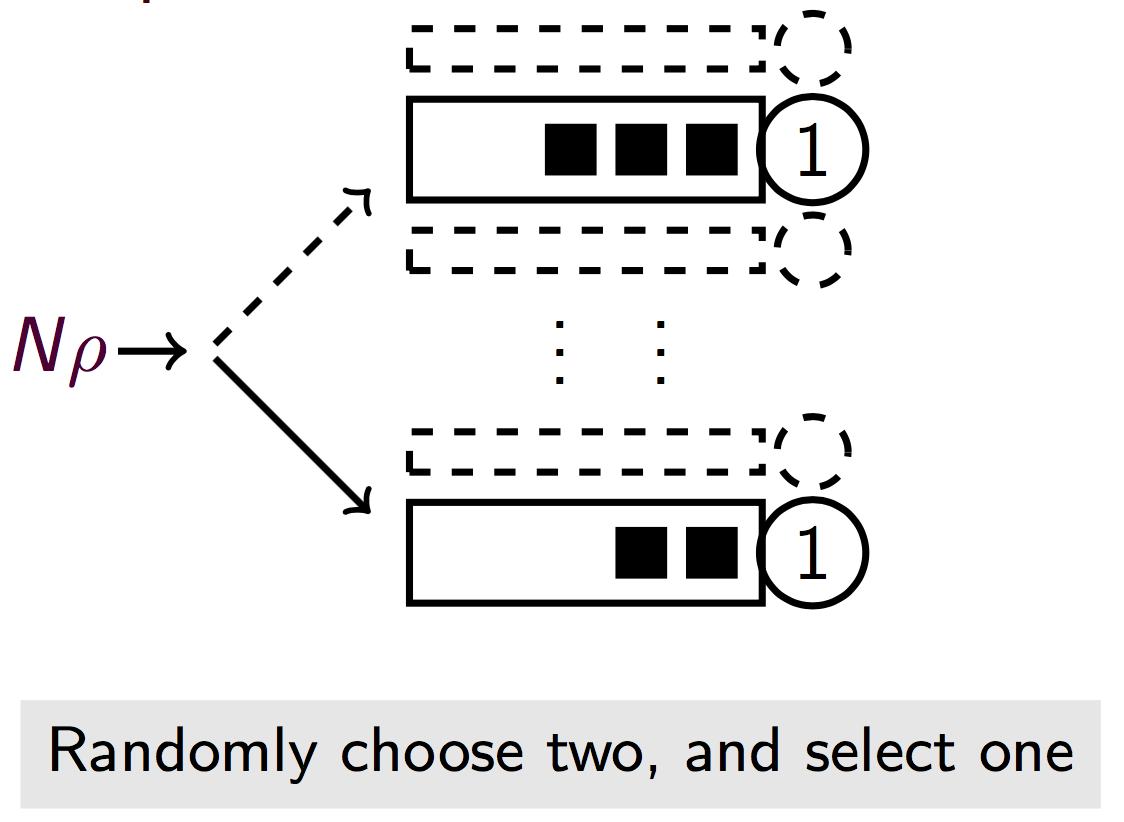
\includegraphics[width=\linewidth]{twoChoiceModel}
    }
    &\mpage{.5}{Infinite state-space:
      \begin{align*}
        X_0(t),X_1(t),\dots
      \end{align*}
      where
      \begin{align*}
        X_i(t) = \text{fraction with $i$ or more jobs}.
      \end{align*}
      }
  \end{tabular}
\end{frame}

\begin{frame}{Does this model satisfies our assumptions? }
  
  $(\bE,\norm{\cdot})$ is the set of infinite sequences such that
  $\norm{x}_w=\sum_{i=1}^\infty w_i\abs{x_i}<\infty$. 

  \begin{itemize}
  \item Transitions : \green{easy}
  \item Regularity of the drift : \green{easy}
  \item Unique attractor : \red{not easy} (mitzenmacher 98),
    exponentially stable 
    : \green{relatively easy} (mitzenmacher 98). 
  \item Stationary measure concentrates on a bounded set :
    \green{relatively easy} (Turner 98) coupling argument : 2-choice
    $\ll$ 1-choice.
  \end{itemize}
\end{frame}


\begin{frame}{The power of two-choice}
  
  
  Our theorem guarantees that the average queue length satisfies:
  \begin{align*}
    m^N(\rho) = m^{\infty}(\rho) + O(1/N),
  \end{align*}
  where  $m^{\infty}(\rho) \approx 
  \log_2\frac1{1-\rho}$ (as $\rho\to1$). 

  \pause\bigskip 
  By simulation, we observe that
  $N(m^N(\rho)-m^{\infty})\to d(\rho)\approx\frac{\rho^2}{2(1-\rho)}$
  \bigskip

  \begin{table}[t]
    \centering
    \begin{tabular}{|c|c|c|c|c|c|}
      \hline
      $N$
      &$  10$  &$  20$  &$  30$  &$  50$ & $+\infty$  \\\hline
      $m^N(\rho)$ [simulation]
      &$2.804$ &$2.566$ &$2.491$ &$2.434$&-- \\\hline $m^\infty(\rho)+\frac{\rho^2}{2N(1-\rho)}$ 
      &$2.758$ &$2.555$ &$2.488$ &$2.434$&$2.353$ \\
      \hline
    \end{tabular}
  \caption{Average queue length in the two-choice model ($\rho=0.9$).}
  \label{tab:2}
\end{table}
  
\end{frame}

\begin{frame}{The quality of the approximation degrades as $\rho$
    goes to $1$}


  Simulation results suggest that: 
  \begin{align*}
    m^N(\rho) \approx \underbrace{m^{\infty}(\rho)}_{\displaystyle\color{red}\approx
    \log_2\frac1{1-\rho}} + \quad \frac1{N}\underbrace{d(\rho)}_{\approx \displaystyle\color{red}
    \frac{\rho^2}{2(1-\rho)}} +\quad O(\frac1{N^2})
  \end{align*}
  \bigskip
  

  \bigskip
  
  Conjecture: the power of two-choice holds if $N = \Omega(\frac1{1-\rho})$
\end{frame}


\section{Recap and Discussion}

\begin{frame}{Recap}
  
  \begin{enumerate}
  \item Convergence of mean-field model is $O(1/N)$. 
    \begin{itemize}
    \item Works for transient and steady-state 
    \item Works for infinite-dimensional state space. 
    \end{itemize}\bigskip
    
  \item Our approach is to focus on the expected values
    \begin{center}
      \hspace{-1cm}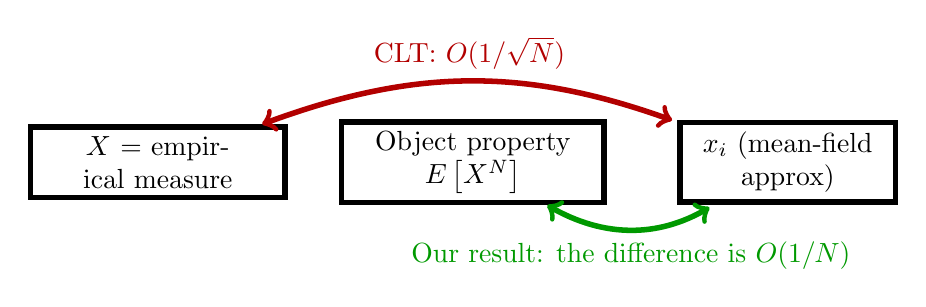
\begin{tikzpicture} \node[text width=3cm,draw,text
        centered] at (0,0) (X) {$X$ = empirical measure}; %
        \node[text width=3.1cm,draw,text centered] at (4,0) (P)
        {Object property\\$\esp{X^N}$}; %
        \node[text width=2.5cm,draw,text centered] at (8,0) (x) {$x_i$
          (mean-field approx)}; \draw[red,line width=2pt] (X)
        edge[bend left,<->,out=20,in=160] node[above]{CLT:
          $O(1/\sqrt{N})$} (x); \draw[green,line width=2pt] (P)
        edge[bend right,<->] node[below]{Our result: the difference is
          $O(1/N)$} (x);
  \end{tikzpicture}
    \end{center}
  \end{enumerate}
\end{frame}

\begin{frame}{In practice}
  For many mean-field models : 
  \begin{align*}
    \esp{X^N} \approx x + \frac{C}{N},
  \end{align*}
  \begin{itemize}
  \item We can estimate $C$
    by simulating one value of $N$ (e.g. $N=100$).
  \item We can use this $C$ to deduce the performance for other values of
    $N$.  
  \end{itemize}
  \bigskip
  
  This provides a new light for the two-choice. 
\end{frame}

\begin{frame}{Does it always work?}
  \begin{itemize}
  \item Works for the model of Kurtz
  \item Also works for the model of \emph{Benaim-Le Boudec 08} by
    using uniformization 
  \end{itemize}

  \bigskip
  But: it requires the drift to be \red{twice-differentiable} (or to
  have a Lipschitz-continuous derivative)
  \begin{itemize}
  \item (see counter-example on the paper)
  \end{itemize}
\end{frame}


\begin{frame}{Extension and open questions}
  \begin{itemize}
  \item Heavy-traffic regime 
  \item Multiple stable equilibria. 
  \item Non-homogeneous population, \emph{e.g.}, caching
  % \item Can we go to the order $O(1/N^2)$? It is useful? 
  % \item Technical conditions (ex: twice-differentiability or
  %   Lipschitz-continuity).
  \end{itemize}
  
  \bigskip\bigskip
  
  Paper, simulations (and slides) are \red{reproducible}:
  \begin{center}
    \url{https://github.com/ngast/meanFieldAccuracy}
  \end{center}
\end{frame}

\appendix

\newcommand\reference[4]{\item[\mpage{.2}{\tiny #1}] \footnotesize 
  \emph{#2}, \tiny #3,  #4}
\begin{frame}{Thank you!}

  %Slides are online at
  \begin{center}
    \url{http://mescal.imag.fr/membres/nicolas.gast}\\ \bigskip
    \texttt{nicolas.gast@inria.fr}
  \end{center}
  \bigskip\bigskip
  
  \qquad\qquad\mpage{.85}{
    Mean-field and decoupling
    \begin{itemize}
      \reference{Bena\"im, \\Le Boudec 08}{A class of mean field
        interaction models for computer and communication
        systems}{M.Bena\"im and J.Y. Le Boudec.}{Performance
        evaluation, 2008.}%
      \reference{Le Boudec 10}{The stationary behaviour of fluid
        limits of reversible processes is concentrated on stationary
        points.}{J.-Y. L. Boudec. }{Arxiv:1009.5021, 2010}%
      \reference{Darling Norris 08}{R. W. R. Darling and
        J. R. Norris}{Differential equation approximations for Markov
        chains}{Probability Surveys 2008} %
      % \reference{Kurtz 70}{}{}{}
      \reference{G. 16}{Construction of Lyapunov functions via
        relative entropy with application to caching}{Gast, N.}{ACM
        MAMA 2016}%
      \reference{G. 16}{Expected Values Estimated via Mean-field
        approximation are $1/N$ accurate}{Gast, N.}{SIGMETRICS 2017}%
      \reference{Budhiraja et al. 15}{Limits of relative entropies
        associated with weakly interacting particle
        systems.}{A. S. Budhiraja, P. Dupuis, M. Fischer, and
        K. Ramanan. }{Electronic journal of probability, 20, 2015.}
    \end{itemize}
  }
\end{frame}

\begin{frame}{References (continued)}
  \qquad\qquad\mpage{.85} {
    Optimal control and mean-field games: 
    \begin{itemize}
      \reference{G.,Gaujal Le Boudec 12}{Mean field for Markov
        decision processes: from discrete to continuous
        optimization}{N.Gast,B.Gaujal,J.Y.Le Boudec}{IEEE TAC, 2012 }%
      \reference{G. Gaujal 12}{Markov chains with discontinuous drifts
        have differential inclusion limits.}{Gast N. and Gaujal
        B.}{Performance Evaluation, 2012} %
      \reference{Lasry Lions}{Mean field games}{J.-M. Lasry and
        P.-L. Lions}{Japanese Journal of Mathematics, 2007.} %
      \reference{Tembine at al 09}{Mean field asymptotics of markov
        decision evolutionary games and teams}{H. Tembine,
        J.-Y. L. Boudec, R. El-Azouzi, and E. Altman.}{GameNets 00}%
    \end{itemize}
    Applications: caches 

    \begin{itemize}
      \reference{Don and Towsley}{An approximate analysis of the LRU
        and FIFO buffer replacement schemes}{A. Dan and
        D. Towsley.}{SIGMETRICS 1990}
      \reference{G. Van Houdt 15}{Transient and Steady-state Regime
        of a Family of List-based Cache Replacement Algorithms.}{Gast,
        Van Houdt.}{ACM Sigmetrics 2015}
    \end{itemize}
  }
\end{frame}

\end{document}
